\chapter{CarryBotsの機構と開発}
本章では,製作した不安定物体を支持可能な車輪型移動ロボットについて述べる.
まず,提案するピニオン車輪&ラックレール機構について述べる.
次に,物体の姿勢を検知するセンサについて述べる.
そして,製作したロボットについて述べる.

\section{ピニオン車輪&ラックレール機構の提案}
前章で述べた式から,上下のロボット間の摩擦を上げることで,物体をより安定に支持することができることがわかった.そこで,それをできる限り大きくするために,ラック・アンド・ピニオン(rack and pinion)機構を採用した.
ロボットにピニオンのような小口径の円形歯車の形の車輪(以下,ピニオン車輪と表記)を利用し,ロボットの上面に歯がつけられたラックの形をしているレール(以下,ラックレールと表記)をつける.ロボットが乗り上げる際に,乗り上げる側のピニオン車輪が乗り上げられる側のラックレールとかみ合わさることで,ロボットは前後にずれることがほとんどなくなり,上下のロボット間の摩擦は非常に大きくなると言える.その他,このピニオン車輪&ラックレール機構を利用すると,ロボットが斜めにずれることを防ぐという利点や,急勾配を登り下りするための推進力と制動力の補助になるという利点が挙げられる.この構造を用いた車輪の外観を\reffig{rack-pinion-concept}に示す.

しかし,地面にあるロボットはピニオン車輪のままで移動すると,ピニオン車輪の歯と地面の接触面積が少ないため,滑りやすいという問題がある.また,とき間が経つと,地面との摩擦でピニオン車輪の歯の摩耗も考えられる.これらの問題を解決するために,\reffig{pinion-wheel-edited}に示すようにピニオン車輪の歯先に滑りにくい,軟質樹脂製パッドをつけることを考えた.これによって,ピニオン車輪のグリップを高める効果が出すことができると,歯の摩耗も解消できると考えられる.

\begin{figure}[tb]
  \centering
  \includegraphics[width=\columnwidth]{./figure/rack-pinion-v2.pdf}
  \caption{Overview of proposal rack-rail and pinion-wheel}
  \label{fig:rack-pinion-concept}
\end{figure}


\begin{figure}[tb]
  \centering
  \includegraphics[width=.8\columnwidth]{figure/elastomer-insert-v2.pdf}
  \caption{3D model of the pinion-wheel and elastomer insert}
  \label{fig:pinion-wheel-edited}
\end{figure}


\section{物体の姿勢を検知するセンサ}
次に,ロボットが物体の姿勢を検知するためのセンサとして,リミットスイッチを採用した.\reffig{limit-switch-edited}に示すように,リミットスイッチを平行に並べると,スイッチの当たり具合で物体の姿勢が推定できると考えられる.例えば,スイッチが二つ同ときに反応した場合,物体は地面に対して垂直であると判定し,下のスイッチだけ反応したら,物体はロボットと反対側に傾いていると判断することができる.リミットスイッチの間の距離を設計することで,物体の傾きの許容範囲を決定することができる.また,物体の傾きを検知する分解能を上げたい場合には,リミットスイッチを数を増やすことで対応することができる.

\begin{figure}[tb]
  \centering
  \includegraphics[width=.5\columnwidth]{figure/posture-detector-v2.pdf}
  \caption{3D model of the posture detector}
  \label{fig:limit-switch-edited}
\end{figure}

\section{実機製作}
前節で設計したピニオン車輪&ラックレールを用いて開発したロボットの外観を\reffig{carrybot}に示す.ロボットの各種パラメータを\reftab{robot-specs}に示す.本体の白色部分と白色のピニオン車輪は3Dプリンタ(X-Smart Qidi Technology製,X-Maker Qidi Technology製)を使ってPLA樹脂を射出成形したものであり,透明部分はTAMIYA製の透明プラバン$0.4$~mmを切り出したものである.透明プラバンの上につけた白色のラックレールは3Dプリンタを使ってTPU(熱可塑性ポリウレタン)を射出成形したものである.ロボットに搭載したマイコン,モータドライバ,モータ,リミットスイッチおよびバッテリーの詳細を以下に示す.また,それらの外観を\reffig{parts}に示す.

\begin{figure}[ht]
  \vspace{0mm}
  \centering
  \begin{tabular}{c}
    \begin{minipage}[ht]{0.5\columnwidth}
      \centering
      \includegraphics[width=\columnwidth]{figure/carrybot-diagonal.pdf}
      \subcaption{Diagonal view}
      \labfig{diagonal-view}
    \end{minipage}
    \begin{minipage}[ht]{0.5\columnwidth}
      \centering
      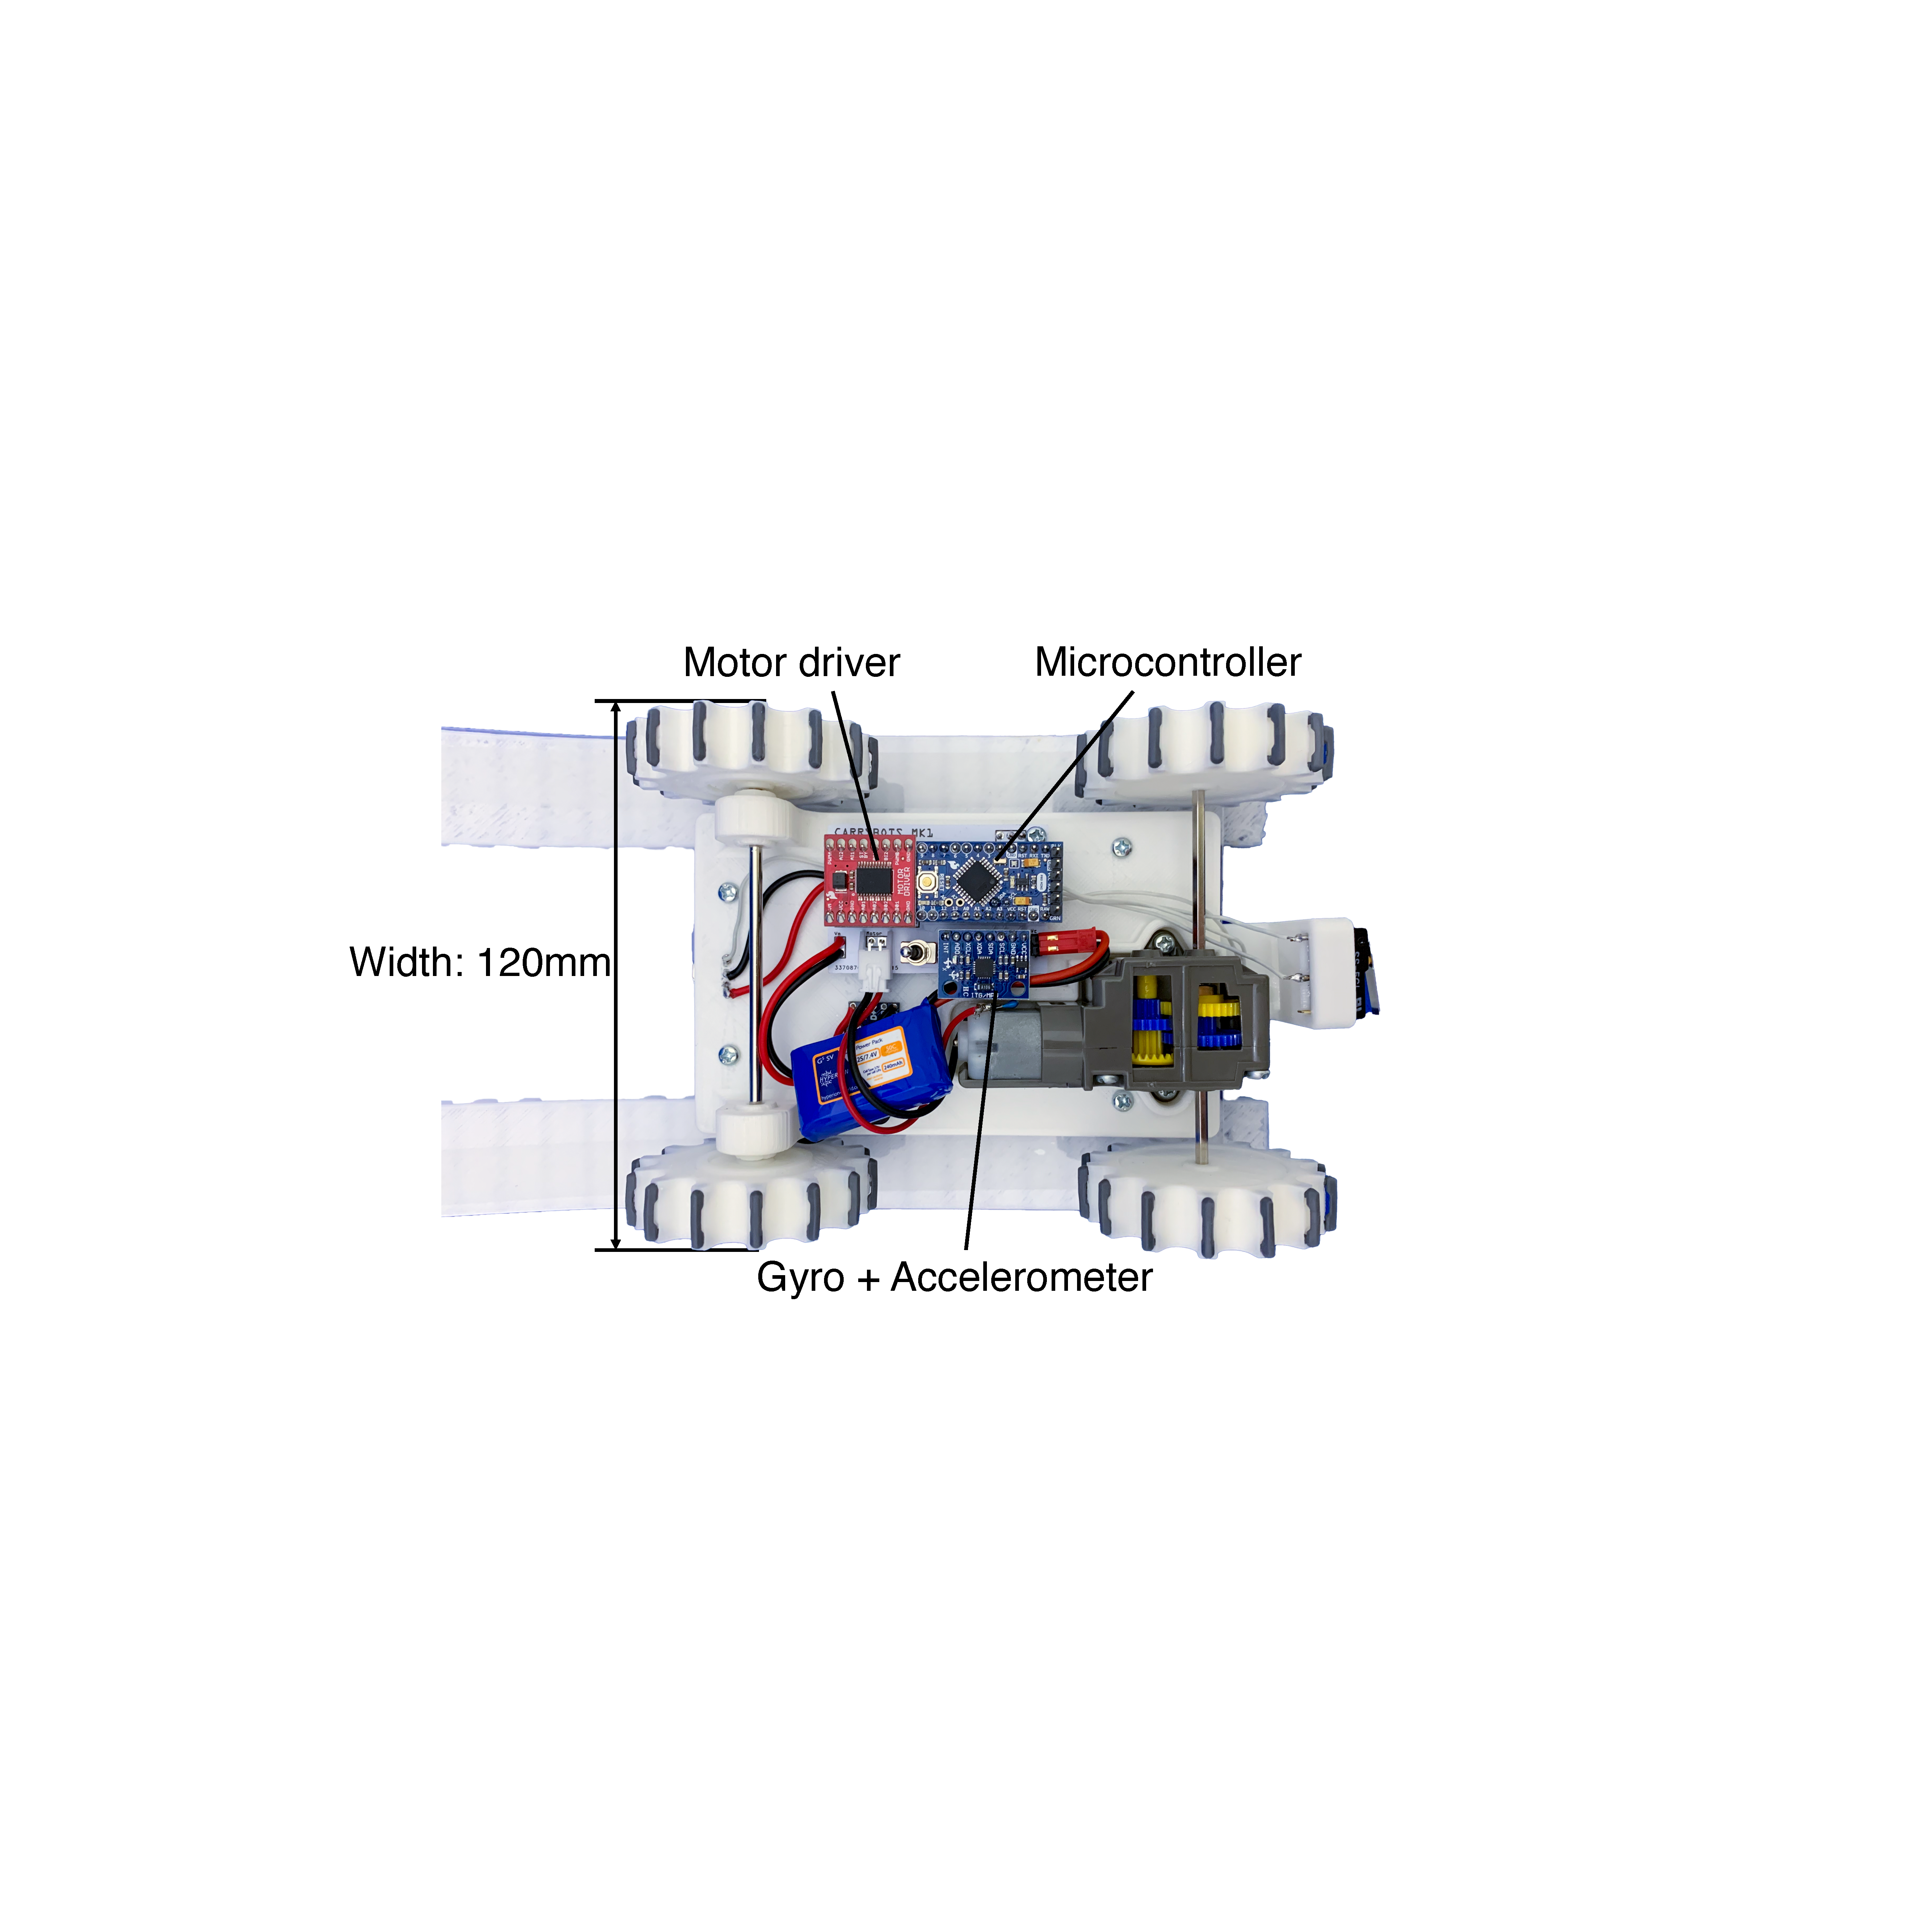
\includegraphics[width=\columnwidth]{figure/carrybot-bottom.pdf}
      \subcaption{Bottom view}
      \labfig{bottom-view}
    \end{minipage}
  \end{tabular}
  \centering
  \caption{Mechanical structure of the developed robot}
  \labfig{carrybot}
\end{figure}


\begin{table}[]
\caption{Specification of the robot}
\centering
\begin{tabular}{ll}
\hline
Weight & 306 g  \\
Width  & 120 mm \\
Length & 250 mm \\
Height & 70 mm  \\ \hline
\end{tabular}
\label{tab:robot-specs}
\end{table}

\begin{figure}[ht]
  \vspace{-9mm}
  \centering
  \begin{tabular}{c}
    \begin{minipage}[ht]{0.4\columnwidth}
      \centering
      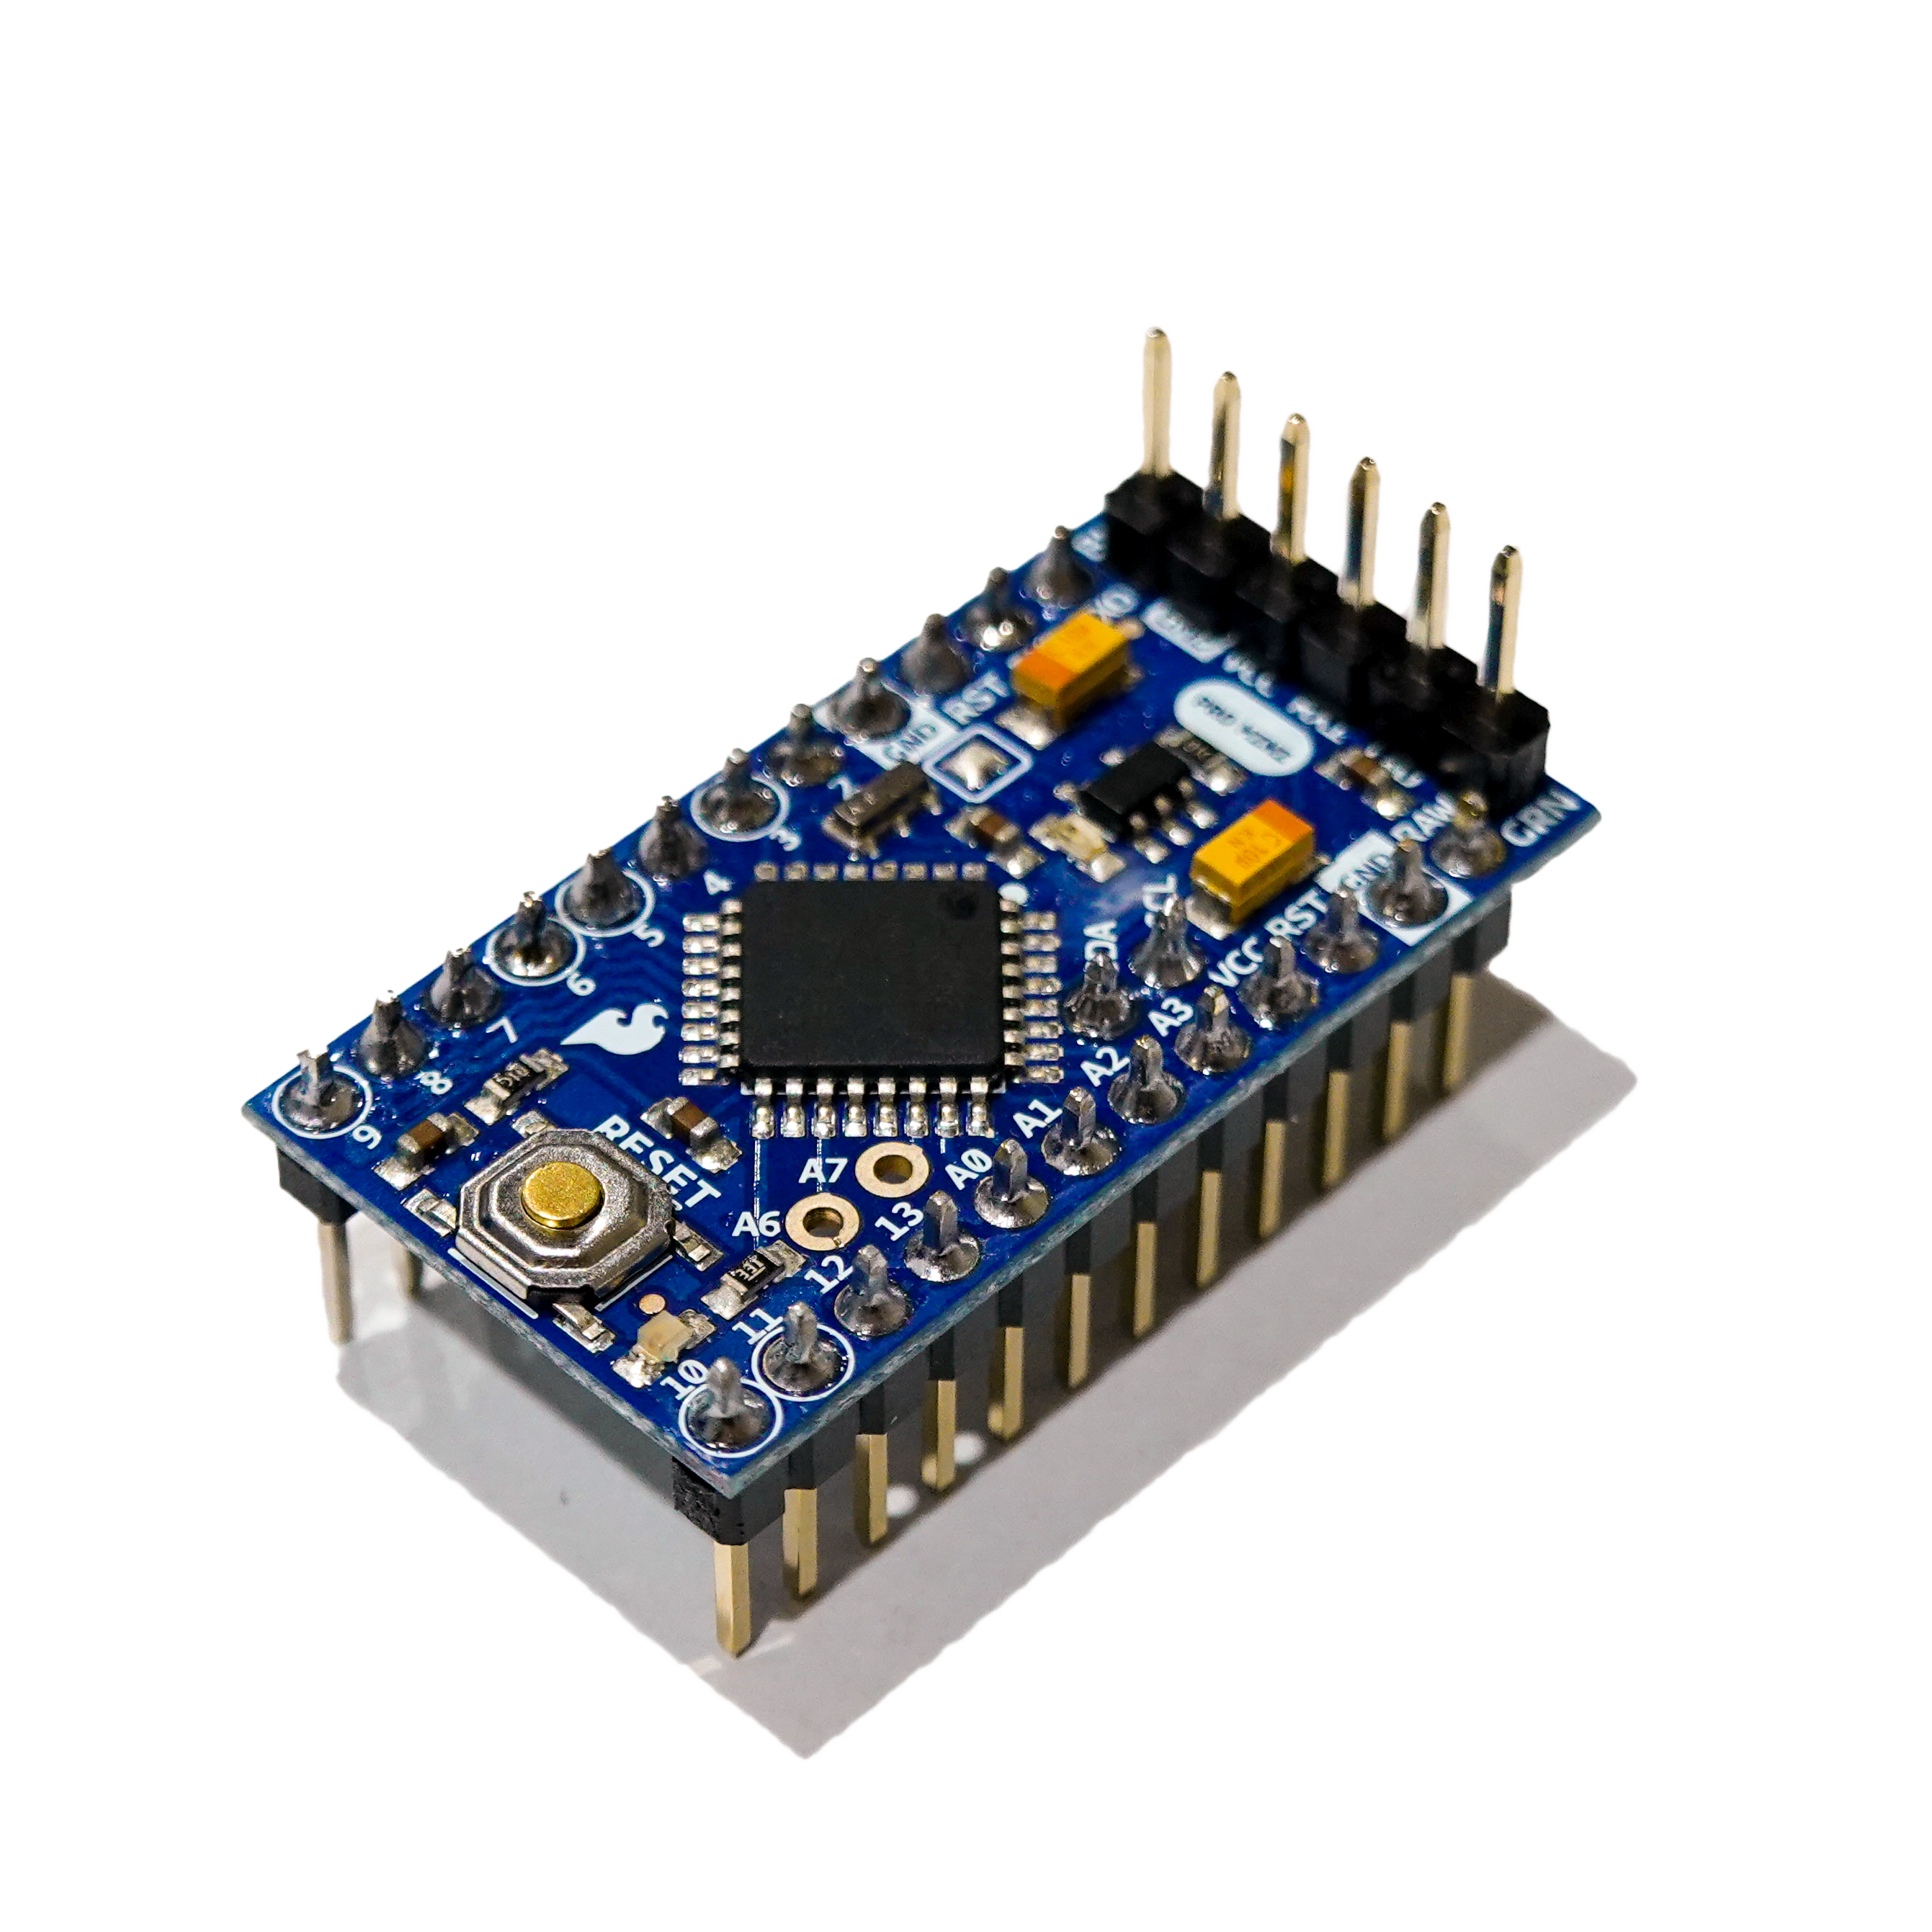
\includegraphics[trim=0 150 0 150, clip,width=0.8\columnwidth]{figure/arduino-pro-mini.png}
      \subcaption{Microcontroller}
      \labfig{arduino}
    \end{minipage}
    \begin{minipage}[ht]{0.4\columnwidth}
      \centering
      \includegraphics[trim=0 150 0 150, clip,width=0.8\columnwidth]{figure/lipo-battery.png}
      \subcaption{LiPo battery}
      \labfig{lipo}
    \end{minipage}\\
    
    \begin{minipage}[ht]{0.4\columnwidth}
      \centering
      \includegraphics[trim=0 150 0 150, clip,width=0.8\columnwidth]{figure/motor-driver.png}
      \subcaption{Motor driver}
      \labfig{motor-driver}
    \end{minipage}
    \begin{minipage}[ht]{0.4\columnwidth}
      \centering
      \includegraphics[trim=0 150 0 150, clip,width=0.8\columnwidth]{figure/DC-motor.png}
      \subcaption{Motor}
      \labfig{motor}
    \end{minipage}\\
    
    \begin{minipage}[ht]{0.4\columnwidth}
      \centering
      \includegraphics[trim=0 150 0 150, clip,width=0.8\columnwidth]{figure/limit-switch.png}
      \subcaption{Limit switch}
      \labfig{limit-switch}
    \end{minipage}
    \begin{minipage}[ht]{0.4\columnwidth}
      \centering
      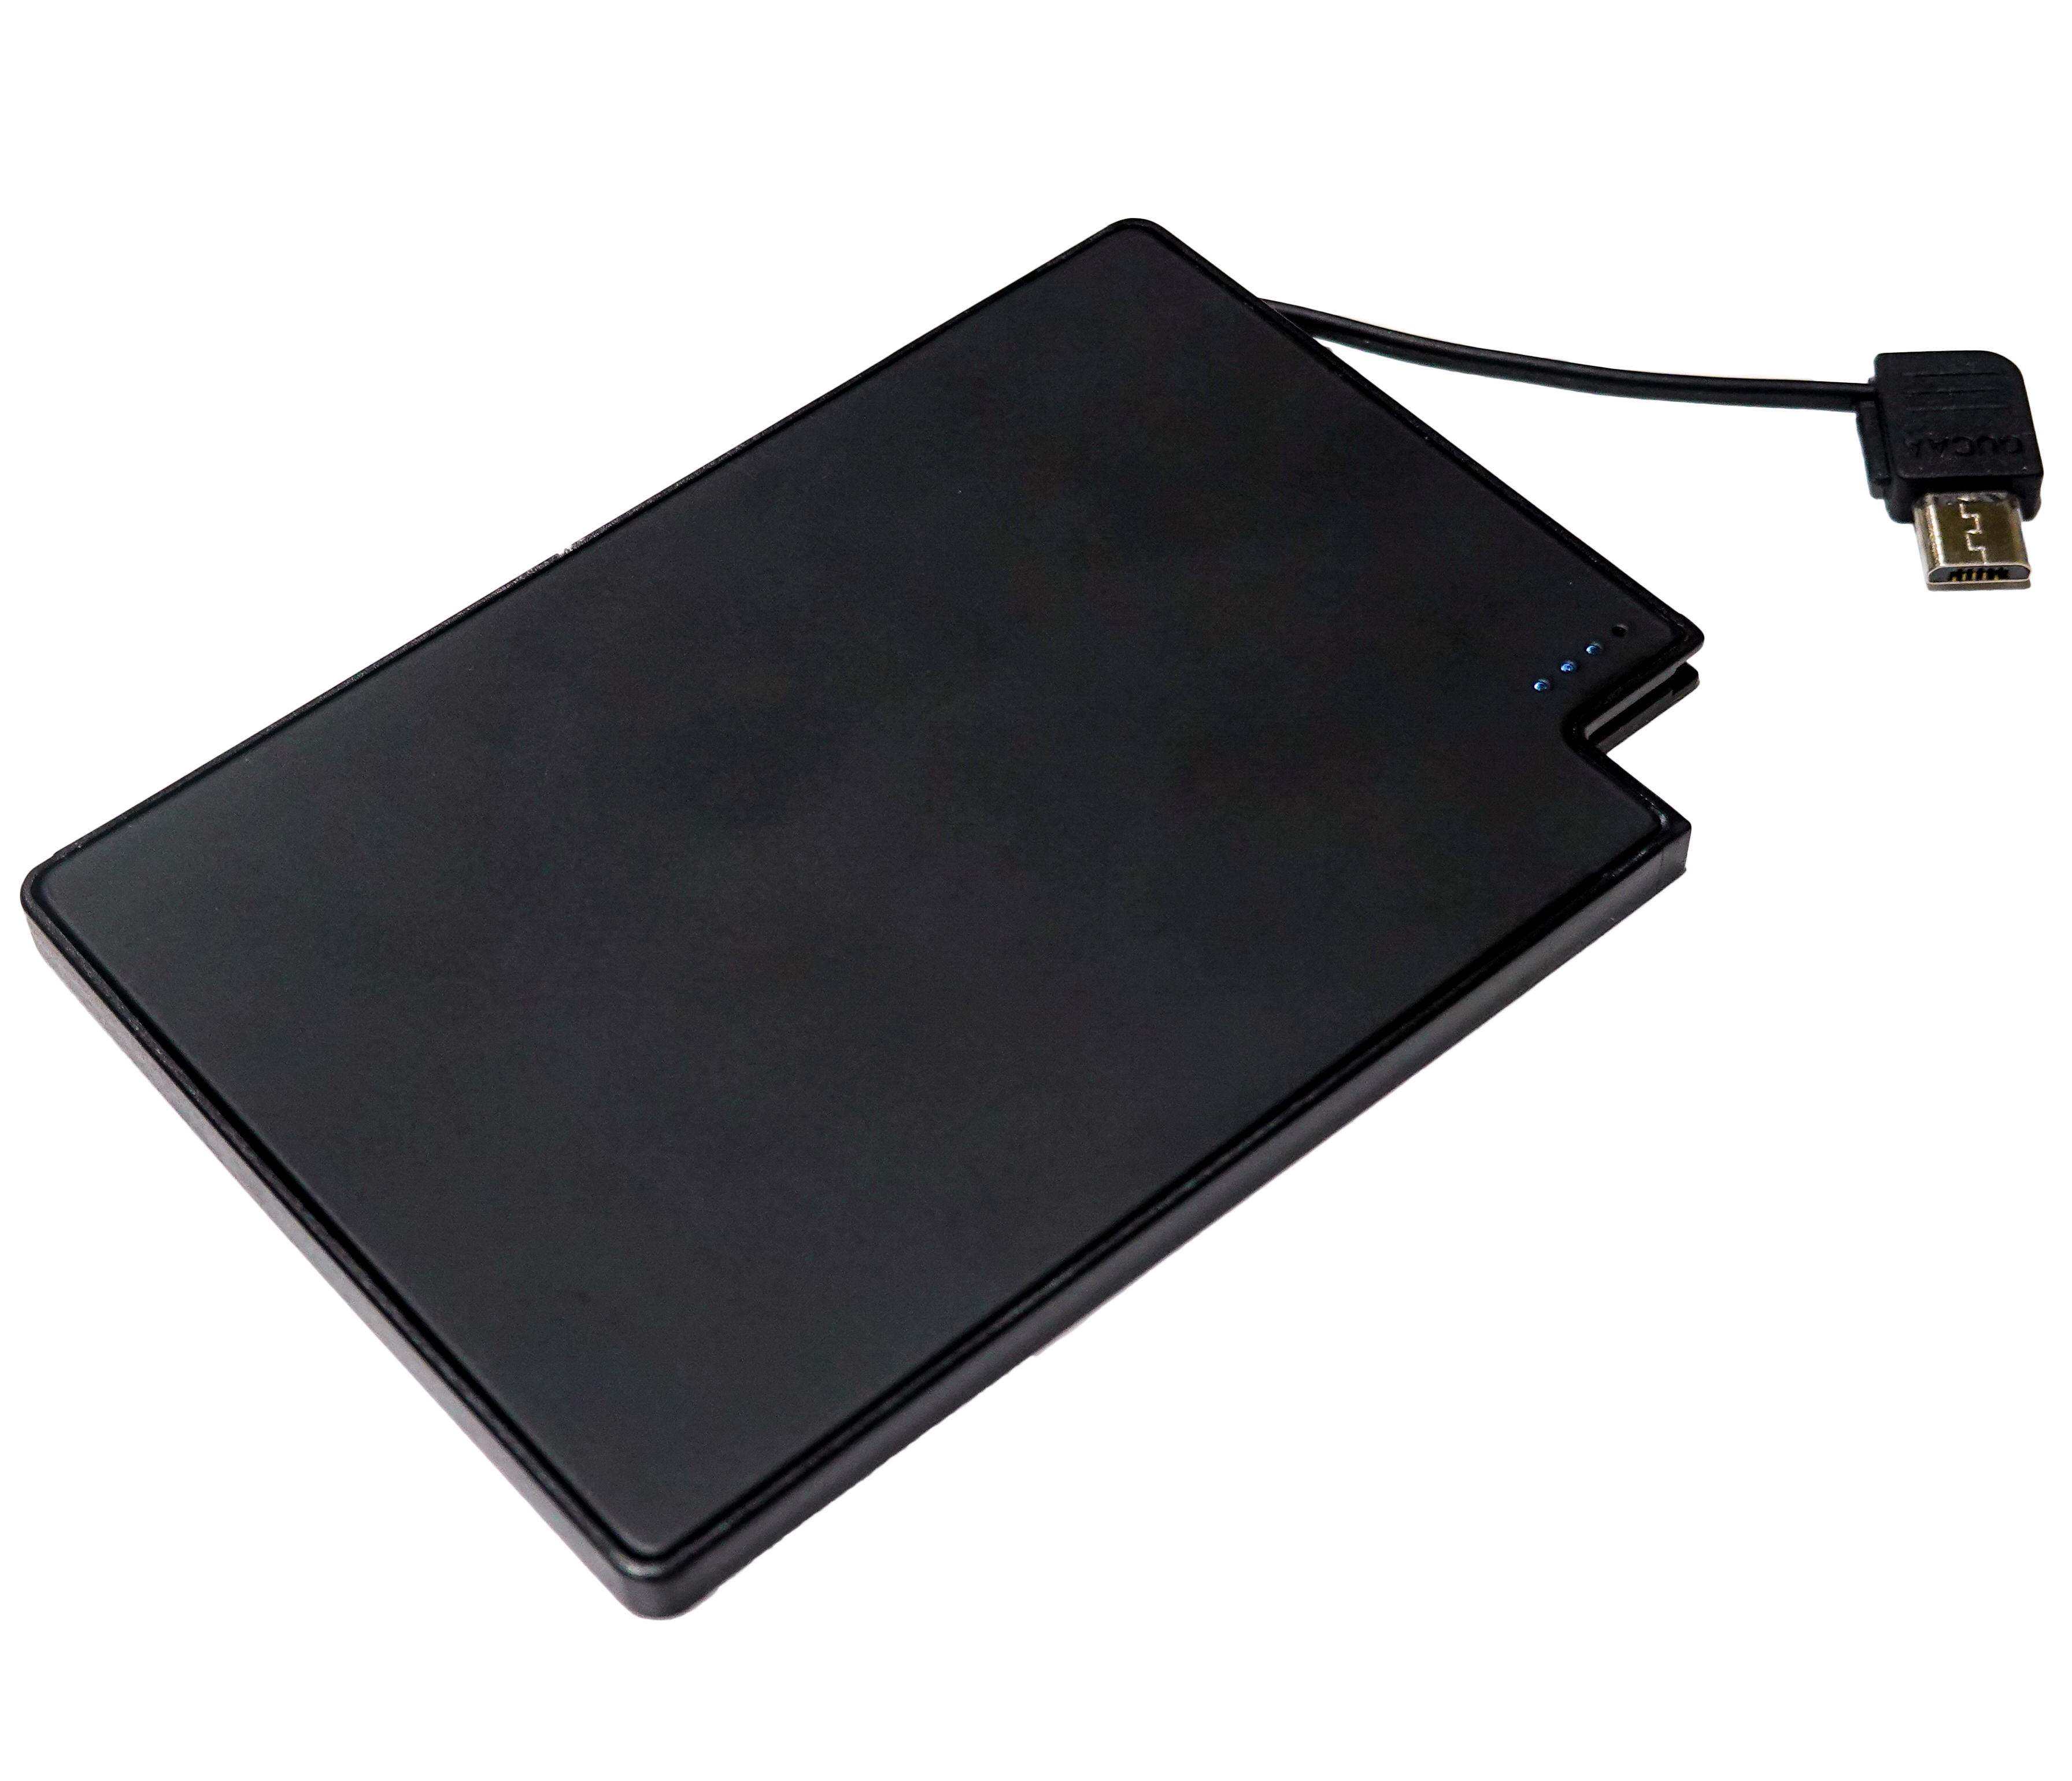
\includegraphics[width=0.8\columnwidth]{figure/mobile-battery.png}
      \subcaption{Power bank}
      \labfig{mobile-battery}
    \end{minipage}\\
    
        \begin{minipage}[ht]{0.4\columnwidth}
      \centering
      \includegraphics[trim=0 150 0 150, clip,width=.8\columnwidth]{figure/mpu6050.png}
      \subcaption{Gyro + Accelerometer}
      \labfig{mpu6050}
    \end{minipage}
    \begin{minipage}[ht]{0.4\columnwidth}
      \centering
      \includegraphics[trim=0 150 0 150, clip,width=.8\columnwidth]{figure/IR-receiver.png}
      \subcaption{IR receiver}
      \labfig{ir-receiver}
    \end{minipage}\\
    
  \end{tabular}
  \centering
  \caption{Overview of experimental instruments}
  \labfig{parts}
\end{figure}

\begin{itemize}
    \item マイコン(Arduino Pro Mini 328 5V 16MHz,SparkFun製) 1個
    \item モータドライバ(Motor Driver-Dual TB6612FNG(1A),SparkFun製) 1個
    \item モータ(FA-130タイプモータ,TAMIYA製)1個
    \item リミットスイッチ(超小型基本スイッチ SS-5GL,オムロン製)2個
    \item 6軸加速度センサージャイロセンサーモジュール(MPU-6050,HiLetgo製)1個
    \item 赤外線リモコン受信モジュール(OSRB38C9AA,OptoSupply製)1個
    \item リチウムイオンポリマー電池(G5 2S 240mAh LiPo 25C(4.2V),Hyperion製) 1個
    \item リチウムイオンポリマー電池(WT-H230 2500mAh(5V),Shenzhen LDTEK Technology Co., Ltd製)1個
\end{itemize}

Arduinoの電源は,リチウムイオンポリマー電池(7.4V)をArduinoに接続し,安定化回路で5Vを得ている.そして,モータの電源はモバイルバッテリー(5V)を使用し,マイクロUSBインターフェイスボード(CJMCU)を通して,給電する.また,赤外線リモコンからの信号を受信しやすくするため,赤外線リモコン受信モジュールを上に向けて,取り付ける.グリップ力を大きくするため,ピニオン車輪の歯先にTAMIYA製の脱着式の軟質樹脂製パッドを取り付ける.

モータはTAMIYA製のシングルギヤボックス(4速タイプ)を用いて,回転速度を$114.7:1$に減速している.モータは1つだけ用いており,左右のクローラーを同じ出力軸に繋ぐことで同量回転させて直進を実現している.ロボットが乗り上げるために,ロボットの後部のプラバンを鉛直下向きに垂れ下がるように曲げ,それをスペーサで挟み,ロボットに取り付ける.また,その上に,ラックレールを両面テープで固定する.これにより,後ろからきた他のロボットのピニオン車輪がラックレールとかみ合わさることで,乗り上げることができる.

